%% Example data sheet
%% Feel free to modify and use this file for any purpose, under
%% either the LaTeX Project Public License or under public domain.

% Options here are passed to the article class.
% Most common options: 10pt, 11pt, 12pt
\documentclass[10pt]{datasheet}

% Input encoding and typographical rules for English language
\usepackage[utf8]{inputenc}
\usepackage[english]{babel}
\usepackage[english]{isodate}

% tikz is used to draw images in this example, but you can
% also use \includegraphics{}.
\usepackage{tikz}
\usepackage{pgfplots}
\usepackage{circuitikz}
\usetikzlibrary{calc}

% These define global texts that are used in headers and titles.
\title{MIPS CPU Data-sheet}
\date{December 2020}

\begin{document}
\maketitle

\section{Overall Architecture}
\smallbreak


\section{Design Decisions}
\smallbreak


% Switch to next column
\vfill\break

\section{Architecture Diagram}
\smallbreak
\begin{figure}[h]
    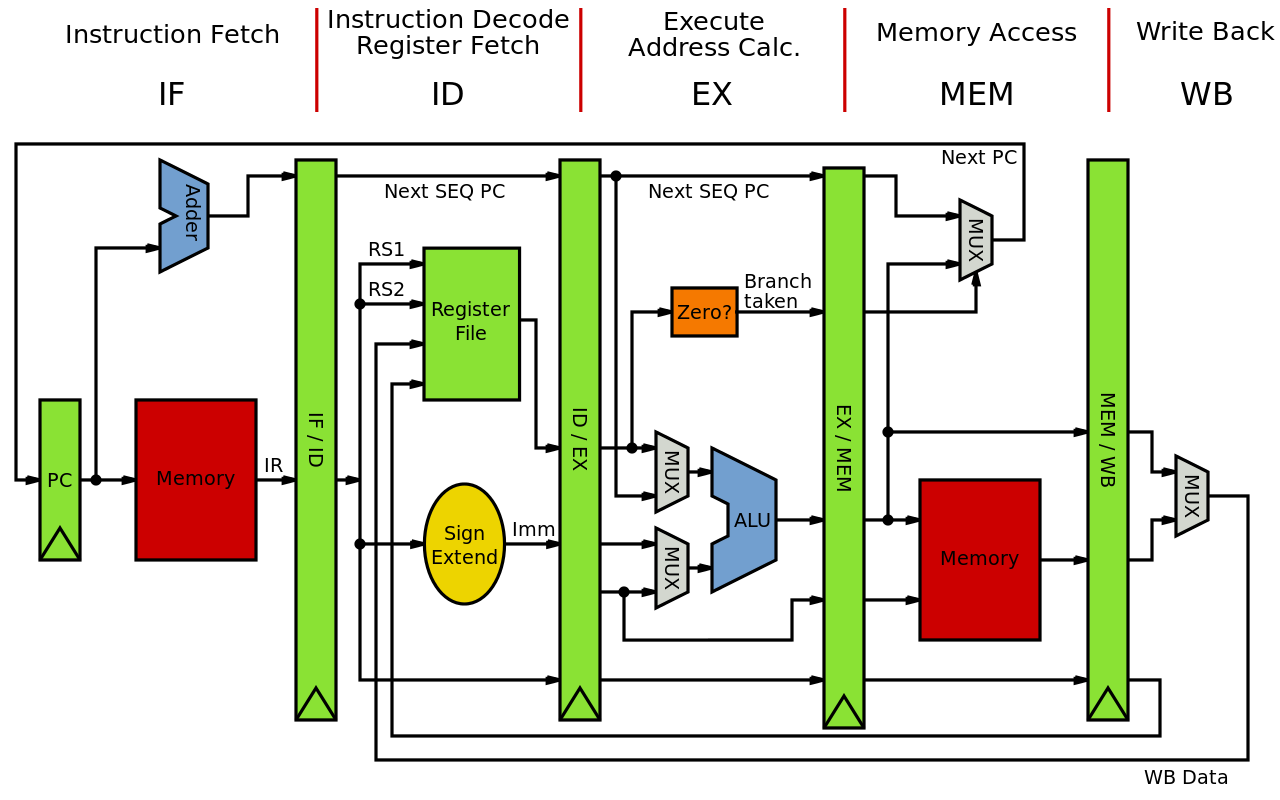
\includegraphics[scale=0.2]{MIPS_Architecture_(Pipelined).svg.png}
    \captionsetup{justification=centering}
    \caption{Mips Pipelined design (Place Holder)}
\end{figure}

Comments on said diagram


% For wide tables, a single column layout is better. It can be switched
% page-by-page.
\newpage

\twocolumn

\section{Testing Approach}
\smallbreak
We choose to do this

\vfill\break

\section{Testing Flow}
Hya


\onecolumn

\section{Area and timing summary}
\smallbreak

\begin{table}[h]
\caption{Summary CPU Specifications}
\begin{tabularx}{\textwidth}{l | c | c c c | c | X}
    \thickhline
    \textbf{Parameter} & \textbf{Symbol} & \textbf{Min.} & \textbf{Typ.} & \textbf{Max.} &
    \textbf{Unit} & \textbf{Conditions} \\
    \hline
    Page width  & $p_w$ & 20.9 & 21.0 & 21.1 & cm & \multirow{2}{*}{Standard A4 paper} \\
    Page height & $p_h$ & 29.6 & 29.7 & 29.8 & cm &  \\
    \hline
    Insulation voltage & $E_{max}$\footnotemark[1] & & 1 & & kV & \\
    \thickhline
\end{tabularx}
\footnotetext[1]{Based on characterization data, not tested in production.}
\end{table}

\textbf{Note:} All measurements taken above were performed in the Cyclone IV E Auto Quartus

\end{document}


